\documentclass[11pt,a4paper]{article}

% --- Paquetes de Estilo y Formato ---
\usepackage[utf8]{inputenc}
\usepackage[spanish,es-tabla]{babel}
\usepackage[T1]{fontenc}
\usepackage{geometry}
\geometry{top=3cm, bottom=3cm, left=3cm, right=2.5cm}
\usepackage{tabularx}
\usepackage{titlesec}
\usepackage{fancyhdr}
\usepackage{lastpage}
\usepackage{hyperref}
\usepackage{enumitem}
\usepackage{graphicx}
\usepackage{tikz}
\usepackage{float}
\usepackage[table, xcdraw]{xcolor}
\usepackage{pdfpages} % PAQUETE NECESARIO PARA INSERTAR EL PDF DE LOS PLANOS

% --- Definición de Colores Corporativos ArthroDesign ---
\definecolor{ArthroNavy}{HTML}{0F172A}
\definecolor{ArthroTeal}{HTML}{0D9488}
\definecolor{ArthroGray}{HTML}{64748B}

% --- Configuración de Párrafo ---
\setlength{\parskip}{0.5em}
\setlength{\parindent}{1.5em}

% --- Estilo de Títulos con Identidad Corporativa ---
\titleformat{\section}
  {\color{ArthroNavy}\Large\bfseries}
  {\thesection.}
  {0.5em}
  {}
  [{\color{ArthroTeal}\titlerule[1.5pt]}]

\titleformat{\subsection}
  {\color{ArthroNavy}\large\bfseries}
  {\thesubsection.}
  {0.5em}
  {}
  [{\color{ArthroTeal}\titlerule[1pt]}]

\titleformat{\subsubsection}
  {\color{ArthroNavy}\large\bfseries}
  {\thesubsubsection.}
  {0.5em}
  {}

% --- Viñetas en color Turquesa ---
\renewcommand{\labelitemi}{\color{ArthroTeal}\textbullet}
\renewcommand{\labelitemii}{\color{ArthroTeal}\circ}

% --- Configuración de Enlaces ---
\hypersetup{colorlinks=true, linkcolor=ArthroNavy, urlcolor=ArthroTeal}

% --- CONFIGURACIÓN DE ENCABEZADO Y PIE CORPORATIVO ---
\pagestyle{fancy}
\fancyhf{}

% Línea superior de color turquesa (Grosor 2pt)
\renewcommand{\headrule}{\hbox to\headwidth{\color{ArthroTeal}\leaders\hrule height 2pt\hfill}}

% Información de Encabezado
\fancyhead[L]{\small \textbf{\color{ArthroNavy}Adaptador ergonómico - PR-PIB-GIS26-09}}
\fancyhead[R]{\small \textbf{\color{ArthroNavy}Documento Nº 4: Planos}}

% Información de Pie de Página (Formato Pág. X de Y incorporado)
\fancyfoot[L]{\small \color{ArthroGray}ArthroDesign Solutions S.L.}
\fancyfoot[C]{\small \color{ArthroGray}\today}
\fancyfoot[R]{\small \textbf{\color{ArthroNavy}Pág. \thepage \ de \pageref{LastPage}}} 

\setlength{\headheight}{15pt}
\renewcommand{\footrulewidth}{0.4pt}

\begin{document}

% ======================================================
% PÁGINA 1: PORTADA
% ======================================================
\begin{titlepage}
    % --- Elementos Geométricos de Identidad (Cabecera y Pie) ---
    \begin{tikzpicture}[remember picture,overlay]
        % Franja superior
        \fill[ArthroNavy] (current page.north west) rectangle ([yshift=-4.5cm]current page.north east);
        \fill[ArthroTeal] ([yshift=-4.5cm]current page.north west) rectangle ([yshift=-4.7cm]current page.north east);
        
        % Franja inferior
        \fill[ArthroNavy] (current page.south west) rectangle ([yshift=2.5cm]current page.south east);
        \fill[ArthroTeal] ([yshift=2.5cm]current page.south west) rectangle ([yshift=2.7cm]current page.south east);
    \end{tikzpicture}

    \centering % Todo centrado a partir de aquí

    % --- LOGO (Sobre la franja azul) ---
    \vspace*{-2cm}
    
\includegraphics[width=6.5cm]{logo_definitivo.png} \\
    \vspace{2cm}

    % --- BLOQUE DE TÍTULO PRINCIPAL ---
    {\color{ArthroGray}\Huge \textbf{DOCUMENTO Nº 4}} \\
    \vspace{0.5cm}
    {\color{ArthroNavy}\Huge \textbf{PLANOS}} \\
    \vspace{0.3cm}
    {\color{ArthroTeal}\rule{12cm}{2pt}} \\
    \vspace{1cm}
    {\Large \textbf{TÍTULO DEL PROYECTO:}} \\
    \vspace{0.3cm}
    {\Huge \bfseries Diseño de un adaptador ergonómico universal para la optimización de la pulsación manual en inhaladores de dosis medida (MDI)} \\
    \vspace{1.3cm}

    % --- BLOQUE DE IDENTIFICACIÓN TÉCNICA ---
    \begin{minipage}{0.8\textwidth}
        \centering
        \textbf{CÓDIGO DE IDENTIFICACIÓN:} \\
        {\large \texttt{PR-PIB-GIS26-09}} \\[0.8cm]
        
        \textbf{PROMOTOR Y EMPRESA DESARROLLADORA:} \\
        {ArthroDesign Solutions S.L.}\\
        {Calle Severo Ochoa, Nº 12, 29590 Málaga, España}\\        
        {NIF:} {B12345678} \\
         
        \href{mailto:contacto@arhtrodesign.com}{contacto@arhtrodesign.com}
    \end{minipage}

    \vspace{1.0cm}

    % --- BLOQUE DE PROYECTISTAS ---
    \textbf{PROYECTISTAS (Equipo de ArthroDesign Solutions S.L.):} \\
    \vspace{0.3cm}
    \small
    \renewcommand{\arraystretch}{1.3}
    \begin{tabular}{l l}
        \textbf{D. Sergio Carmona Muñoz} & Colegiado Nº 06424 (DNI: 26291930D) \\
        \textbf{D. Juan Gabriel Navarro Valdivielso} & Colegiado Nº 06425 (DNI: 77666662D) \\
        \textbf{D. Antonio Sánchez Doña} & Colegiado Nº 06423 (DNI: 79380534J) \\
        \textbf{D. Iván de la Torre Segato} & Colegiado Nº 06421 (DNI: 79383630G) \\
    \end{tabular}
    
    \vfill

    % --- PIE DE PORTADA ---
    {\color{white} ArthroDesign Solutions S.L. \quad | \quad \today}
    \vspace{-1.75cm} 
\end{titlepage}

% AÑADE ESTA LÍNEA AQUÍ PARA QUE LA SIGUIENTE PÁGINA SEA LA 2:
\setcounter{page}{2}

% ======================================================
% HOJA EN BLANCO CON MARCA DE AGUA
% ======================================================
\newpage
\pagestyle{fancy}

\begin{tikzpicture}[remember picture, overlay]
    \node[opacity=0.1] at (current page.center) {
\includegraphics[width=12cm]{logo_definitivo.png}};
\end{tikzpicture}

% Empujamos el texto hacia la parte inferior del folio
\vspace*{8.5cm} 
\begin{center}
    \textit{Esta hoja ha sido dejada deliberadamente en blanco.}
\end{center}
\vfill
\newpage

% ======================================================
% PÁGINA: ÍNDICE GENERAL DE PLANOS Y FIRMAS
% ======================================================
\section*{ÍNDICE DE PLANOS}
\addcontentsline{toc}{section}{Índice General de Planos}
\vspace{0.6cm}

% Índice normalizado con puntos de tabulación y número de página
\begin{itemize}[label={}, leftmargin=0.5cm, itemsep=0.8em]
    \item \textbf{Plano Nº 1.} Plano General \dotfill 4
    \item \textbf{Plano Nº 2.} Plano Explosionado\dotfill 5
    \item \textbf{Plano Nº 3.} Plano de la Base \dotfill 6
    \item \textbf{Plano Nº 4.} Plano del Pivote \dotfill 7
    \item \textbf{Plano Nº 5.} Plano de la Palanca\dotfill 8
\end{itemize}

\vspace{2.5cm}

% ======================================================
% BLOQUE DE FIRMAS (Precede a los planos formales)
% ======================================================
\noindent\begin{minipage}{\textwidth}
    \begin{flushright}
        En Málaga, a \today
    \end{flushright}
    \vspace{2cm}

    \noindent
    \begin{minipage}[t]{0.45\textwidth}
        \centering
        \rule{6cm}{0.6pt} \\
        \textbf{Fdo. D. Sergio Carmona Muñoz} \\
        Colegiado Nº 06424 \\
        DNI: 26291930D
    \end{minipage}
    \hfill
    \begin{minipage}[t]{0.45\textwidth}
        \centering
        \rule{6cm}{0.6pt} \\
        \textbf{Fdo. D. Juan Gabriel Navarro Valdivielso} \\
        Colegiado Nº 06425 \\
        DNI: 77666662D
    \end{minipage}

    \vspace{2cm}

    \noindent
    \begin{minipage}[t]{0.45\textwidth}
        \centering
        \rule{6cm}{0.6pt} \\
        \textbf{Fdo. D. Antonio Sánchez Doña} \\
        Colegiado Nº 06423 \\
        DNI: 79380534J
    \end{minipage}
    \hfill
    \begin{minipage}[t]{0.45\textwidth}
        \centering
        \rule{6cm}{0.6pt} \\
        \textbf{Fdo. D. Iván de la Torre Segato} \\
        Colegiado Nº 06421 \\
        DNI: 79383630G
    \end{minipage}
\end{minipage}
\newpage

% ======================================================
% INSERCIÓN DEL PDF CON LOS PLANOS
% ======================================================
% El comando \includepdf inserta las páginas del archivo directamente.
% El parámetro "pages=-" le indica que incluya todas las páginas desde la primera a la última.
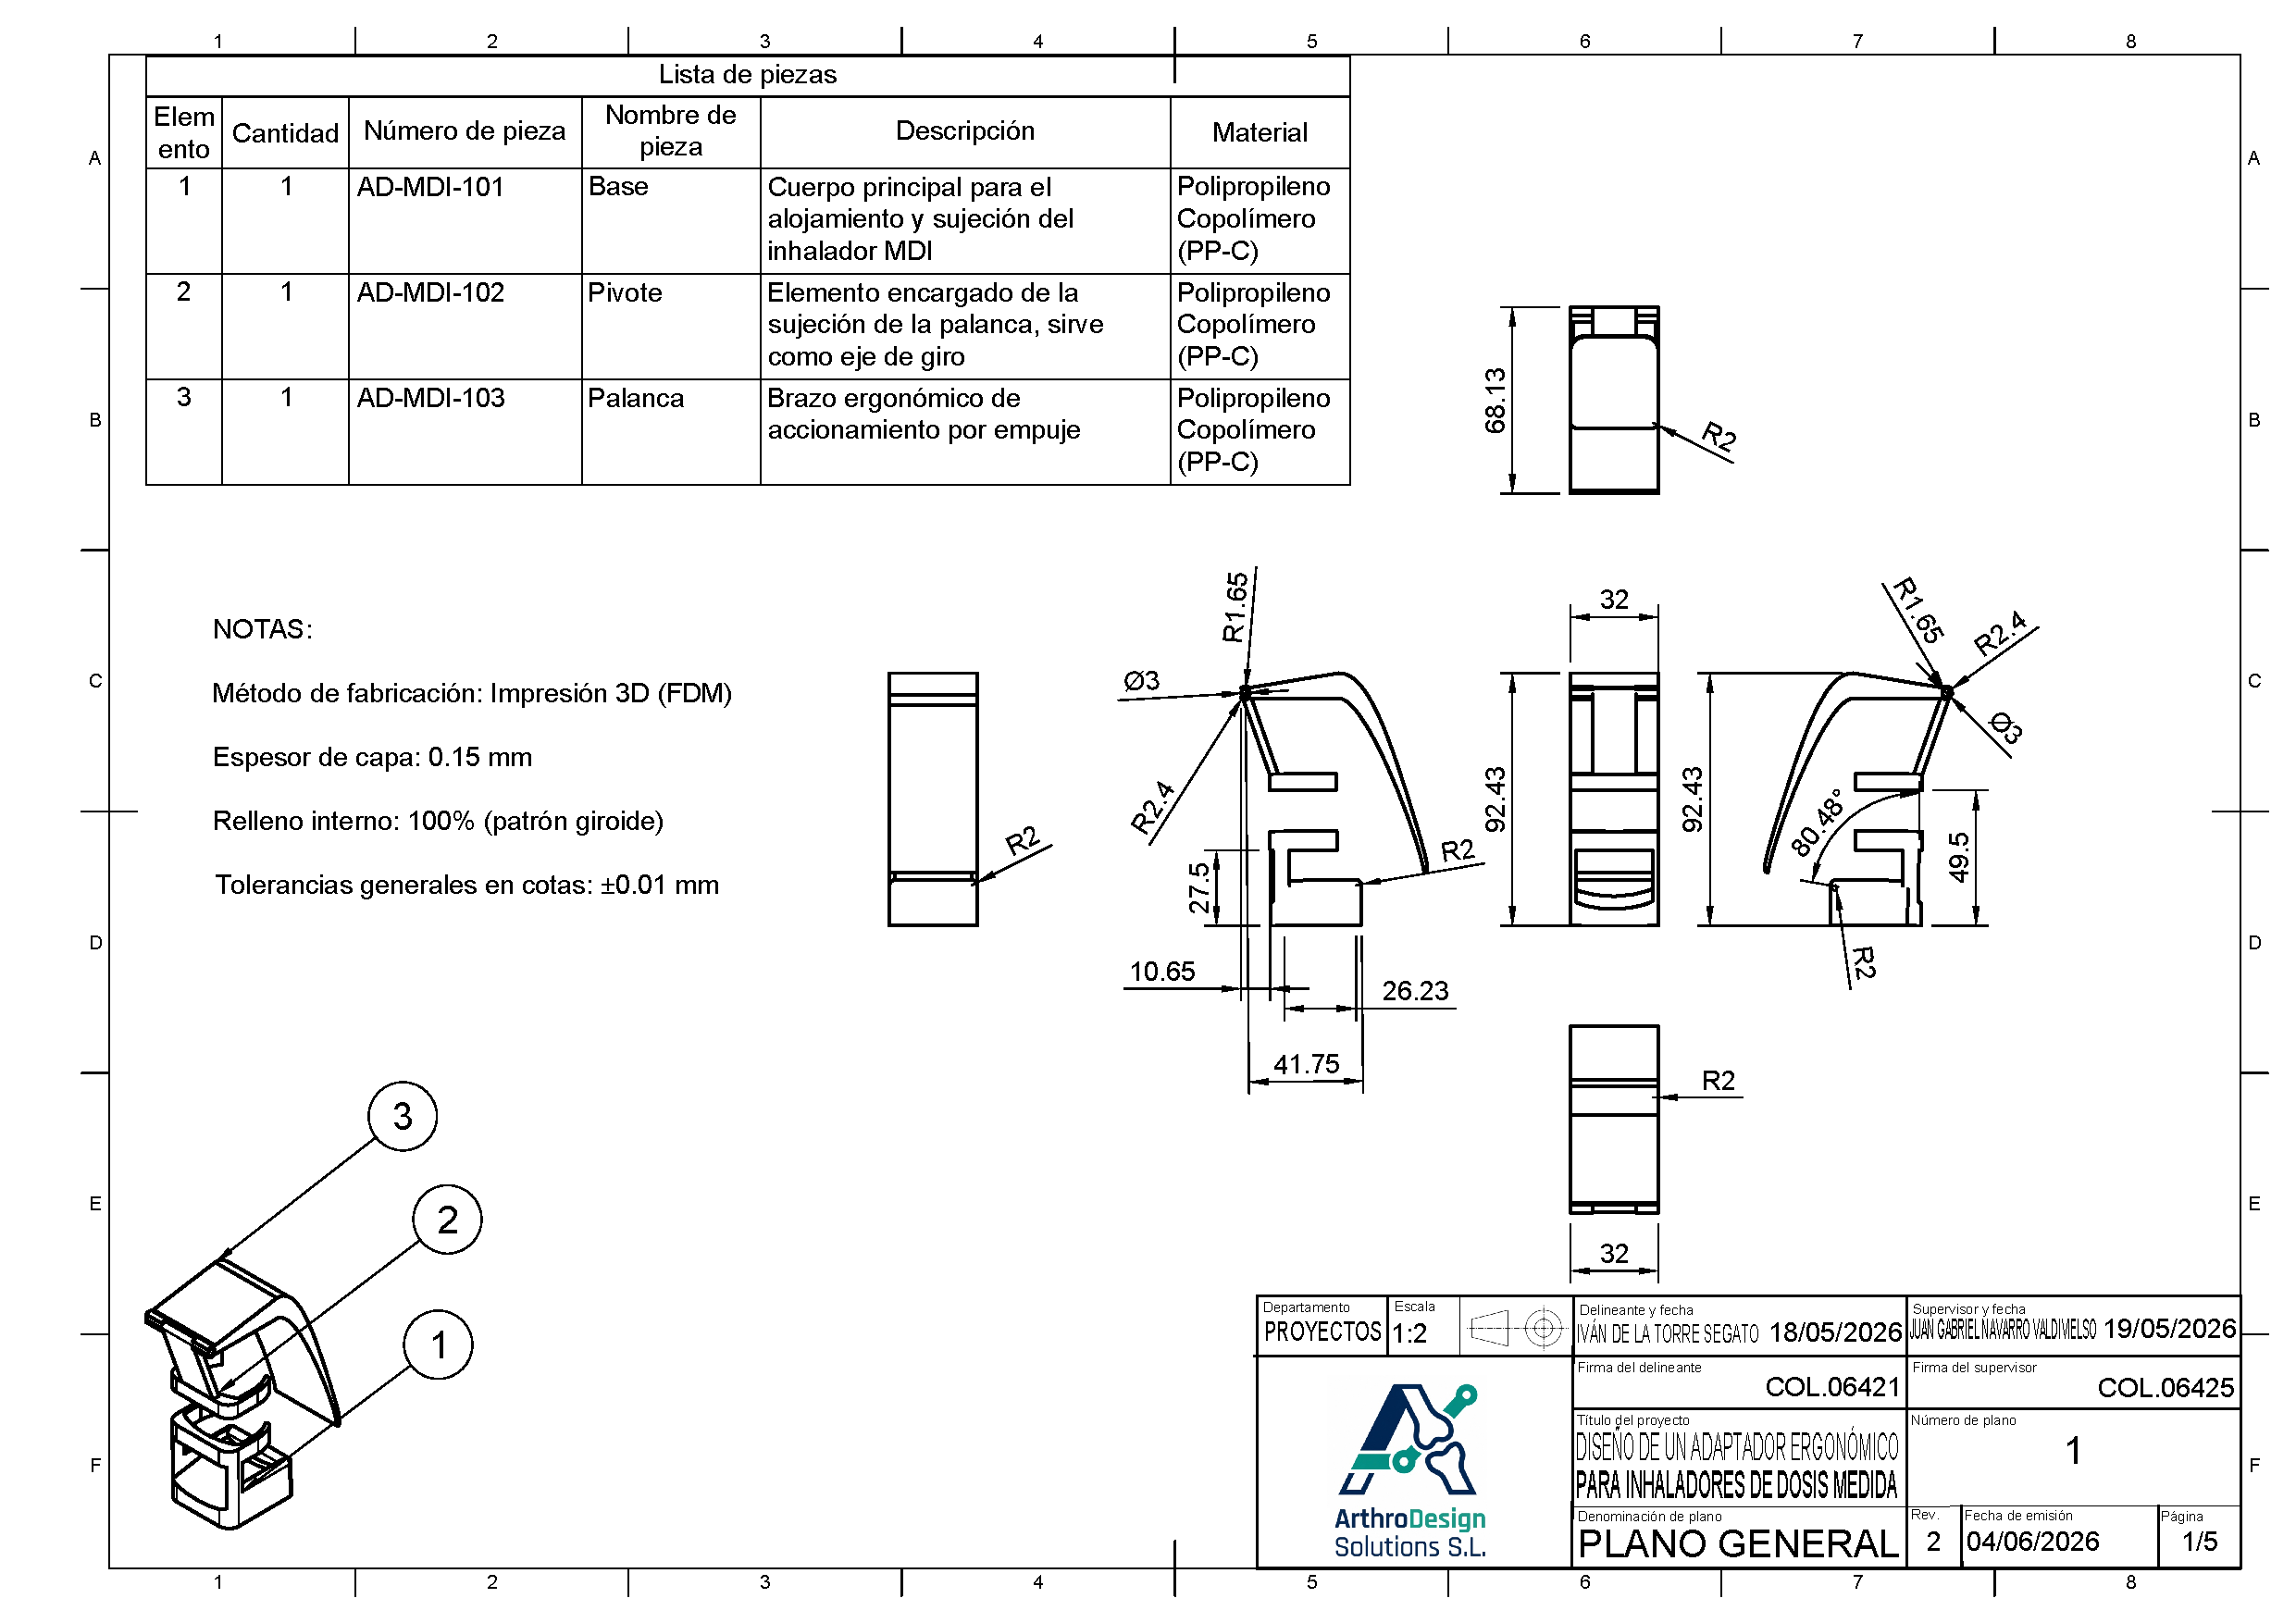
\includepdf[pages=-, fitpaper=true]{PLANOS.pdf}

% ======================================================
% HOJA EN BLANCO CON MARCA DE AGUA
% ======================================================
\newpage
\pagestyle{fancy}

\begin{tikzpicture}[remember picture, overlay]
    \node[opacity=0.1] at (current page.center) {
\includegraphics[width=12cm]{logo_definitivo.png}};
\end{tikzpicture}

% Empujamos el texto hacia la parte inferior del folio
\vspace*{8.5cm} 
\begin{center}
    \textit{Esta hoja ha sido dejada deliberadamente en blanco.}
\end{center}
\vfill

\end{document}